\documentclass[11pt,letter]{article}
\usepackage[top=0.65in,bottom=0.9in,left=0.85in,right=0.85in]{geometry}

%\def\baselinestretch{1.25}
\def\baselinestretch{1.0}

\usepackage[greek, english]{babel}
\usepackage{multicol}

\usepackage{graphicx}
\usepackage[export]{adjustbox}


% The use of the times package forces the use of the type-1 times
% roman font, but the times roman font does not look nice.
% Besides the times roman font still does not print correctly on
% the dopy printer.
%\usepackage{times}


\usepackage{fancyhdr}
\usepackage{amsmath}
\usepackage{amssymb}
\usepackage{bm}
\usepackage{bbold}
\usepackage{parskip}

\newcommand{\bv}[1]{\ensuremath{\bm{#1}}}
\newcommand{\vo}{\ensuremath{V_{0}}}
\newcommand{\er}{\ensuremath{E_{R}}}
\newcommand{\Lc}{\ensuremath{L_{\mathrm{c}}}}
\newcommand{\dsig}[1]{\ensuremath{ \frac{ d\,\sigma_{#1} }{d\,\Omega} }}
\newcommand{\dbl}{\ensuremath{ \uparrow\! \downarrow \, }}
\newcommand{\spup}{\ensuremath{ \uparrow }}
\newcommand{\spdn}{\ensuremath{ \downarrow}}

\begin{document}

\section{One-dimensional optical lattice potential}

The contents of this section follow the derivation found in Sec.~IV~A of \cite{RevModPhys.78.179}.

The Hamiltonian for an atom moving in a 1D lattice potential is 
\begin{equation}
  H_{\text{single,1D}} = - \frac{\hbar^{2}}{2m} \frac{\partial^{2}}{\partial x^{2}} + \vo\cos^{2}(kx) 
\end{equation}
where $k=2\pi/\lambda$, and $\lambda$ is the wavelength of the lattice laser. 
If \vo\ is in units of the recoil energy $\er=\frac{\hbar^{2}k^{2}}{2m}$, then the Hamiltonian is 
\begin{equation}
\begin{split}
  H_{\text{single,1D}}= &-\frac{1}{k^{2}} \frac{\partial^{2}}{\partial x^{2}} + \vo\cos^{2}(kx) \\
  H_{\text{single,1D}} = &-\frac{1}{k^{2}} \frac{\partial^{2}}{\partial x^{2}} + \frac{\vo}{4}(2+e^{2ikx} + e^{-2ikx} )  \\
\end{split}
\end{equation}
The solution to this equation can be found in terms of Bloch states, which are labeled by their quasimomentum $q$, and their band index $n$
\begin{equation}
  \psi_{q}^{n}(x) = e^{iqx} \sum_{m=-\infty}^{\infty} c_{qm}^{n} e^{imGx}
  \label{eq:blochstate}
\end{equation}
The lattice translation invariant function that typically accompanies $e^{iqx}$
has been written here as a sum of plane waves (labeled by the integer $m$) at the reciprocal lattice
vectors.  This is the Fourier series of any such periodic function and represents no loss of
generality.   The reciprocal lattice vector  $G=\frac{2\pi}{a}=2k$,
where $a=\lambda/2$ is the lattice spacing.  

Plugging the Bloch states into the Hamiltonian and then rearranging some of the terms in the infinite sum, we get 
\begin{equation}
\begin{split}
  H_{\text{single,1D}} \psi_{q}(x) = &  \sum_{m} \left[(q/k+2m)^{2} + \frac{\vo}{4}(2+e^{2ikx}+e^{-2ikx}) \right]
                     c_{qm}^{n} e^{iqx+im2kx} \\ 
  H_{\text{single,1D}} \psi_{q}(x) = &  \sum_{m} \left[ \left(  (q/k+2m)^{2} + \frac{\vo}{2} \right) c_{qm}^{n} 
                                     + \frac{\vo}{4}c_{q,m-1}^{n} + \frac{\vo}{4}c_{q,m+1}^{n} \right] 
                     e^{iqx+im2kx} 
\end{split}
\end{equation}
The left hand side of the time-independent Schrodinger equation is simply 
\begin{equation}
  E_{q}^{n}\psi_{q}(x) = \sum_{m} E_{q} c_{qm}^{n} e^{iqx+imGx}
\end{equation}
For the coefficients $c_{qm}^{n}$ to represent an eigenstate of the problem, the
Bloch state needs to satisfy $H\psi_{q}(x) = E_{q}^{n}\psi_{q}(x)$, and since the
plane waves are linearly independent functions this means that 
\begin{equation}
  \left(  (q/k+2m)^{2} + \frac{\vo}{2} \right) c_{qm}^{n} 
                                     + \frac{\vo}{4}c_{q,m-1}^{n} + \frac{\vo}{4}c_{q,m+1}^{n} = E_{q} c_{qm}^{n} 
\end{equation}
From now on we simply express the quasimomentum in units of $k$, so that it takes values in $(-1,1]$.  We have a linear system of equations which determines the $c_{qm}^{n}$.  The number of equations is infinite, but for our practical purposes we will truncate it such that $|m|<\mathcal{N}$.  The resulting equations can be written in matrix form, for example if we select $\mathcal{N}=2$
\begin{equation}
  \left[\begin{smallmatrix}\frac{1}{2} V_{{0}} + \left(q -4\right)^{2} & \frac{1}{4} V_{{0}} & 0 & 0 & 0\\\frac{1}{4} V_{{0}} & \frac{1}{2} V_{{0}} + \left(q -2\right)^{2} & \frac{1}{4} V_{{0}} & 0 & 0\\0 & \frac{1}{4} V_{{0}} & \frac{1}{2} V_{{0}} + q^{2} & \frac{1}{4} V_{{0}} & 0\\0 & 0 & \frac{1}{4} V_{{0}} & \frac{1}{2} V_{{0}} + \left(q + 2\right)^{2} & \frac{1}{4} V_{{0}}\\0 & 0 & 0 & \frac{1}{4} V_{{0}} & \frac{1}{2} V_{{0}} + \left(q + 4\right)^{2}\end{smallmatrix}\right]
\end{equation}
In the numerical solution that  we implemented we chose $\mathcal{N}=5$,  it
turns out that to accurately obtain the dispersion relationship for the
$n^\mathrm{th}$ band you pretty much only need $\mathcal{N}=n+1$, so using
$\mathcal{N}=5$ is somewhat overkill for us since we will be mostly
concentrated on the lowest band and the first excited band.  

\subsection{Band structure}

We can find the solutions for the set of coefficients $c_{qm}^{n}$ by
diagonalizing the matrix shown above.  The eigenvalues correspond to the
energies $E_{q}^{n}$ as a function of quasimomentum $q$ and band index $n$,
this set of solutions is referred to as the band structure, and we show it for
a 1D lattice as a function of $q$ in Fig.~\ref{fig:bands1d}, and also as a function of lattice depth in Fig.~\ref{fig:bands1d_V0}
\begin{figure}
\centering 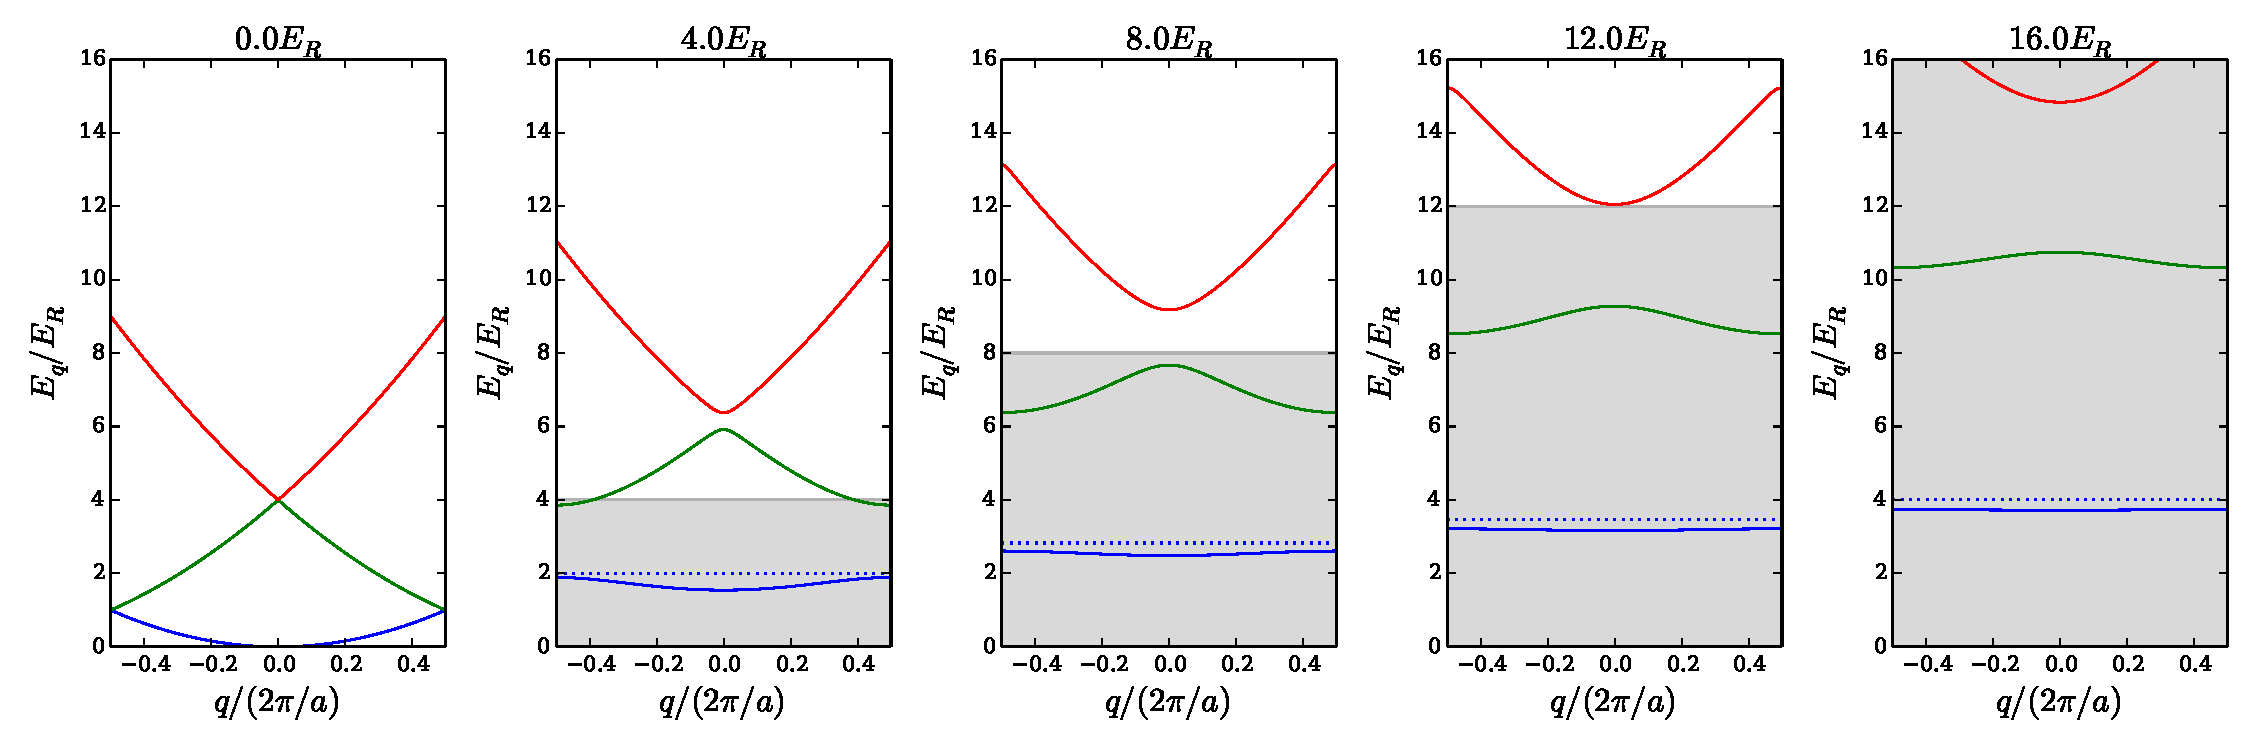
\includegraphics[width=\textwidth]{../BandStructure_figures/bands1d.pdf}
\caption[Band structure in 1D lattice.]{\small Band structure in a 1D optical lattice.  The depth of the lattice is indicated by the shaded area, and the energy of the hamonic oscillator ground state in a single lattice site is shown as a dotted line.  }
\label{fig:bands1d}
\end{figure}
\begin{figure}
\centering 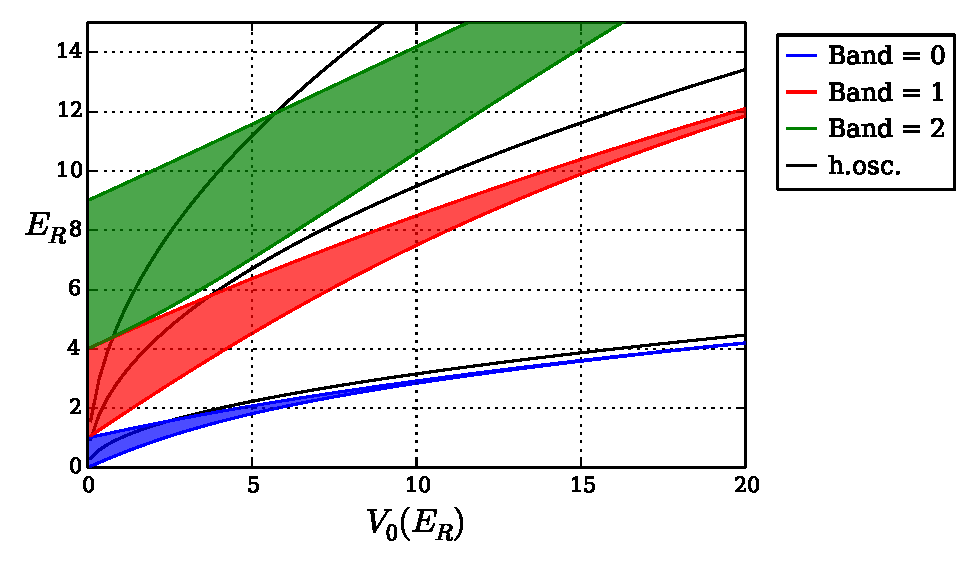
\includegraphics[width=0.6\textwidth]{../BandStructure_figures/bands1d_V0.pdf}
\caption[Band structure in 1D lattice.]{\small Band structure in a 1D optical lattice.  Each band is indicated by the colored area,  the harmonic oscillator states in an isolated lattice site are shown as black lines. }
\label{fig:bands1d_V0}
\end{figure}

\subsection{Eigenstates}
For each energy eigenvalue we have
an associated eigenstate  which is defined in terms of the
$c_{qm}^{n}$ by Eq.~\ref{eq:blochstate}.   Typically, numerical diagonalization routines return the normalized eigenvectors of the matrix in question,  and for us this means that the coefficients $c_{qm}^{n}$ will satisfy
\begin{equation}
   \sum_{m} | c_{qm}^{n} |^{2} = 1 
\end{equation} 
This has the implication that the states obtained from Eq.~\ref{eq:blochstate} will be normalized over a lattice site.  In Fig.~\ref{fig:eigenfuns1d}. we
show the probability density for a lowest band eigenstate as a function of
position in the lattice for various lattice depths.  One can see how as the
lattice gets deeper the state becomes more localized around the center of each
lattice site. Notice that the sites are the positions where $x/a$ is a half-integer, this is due to the fact that we have chosen $\vo>0$ and a cosine to represent the lattice potential.  
\begin{figure}
\centering 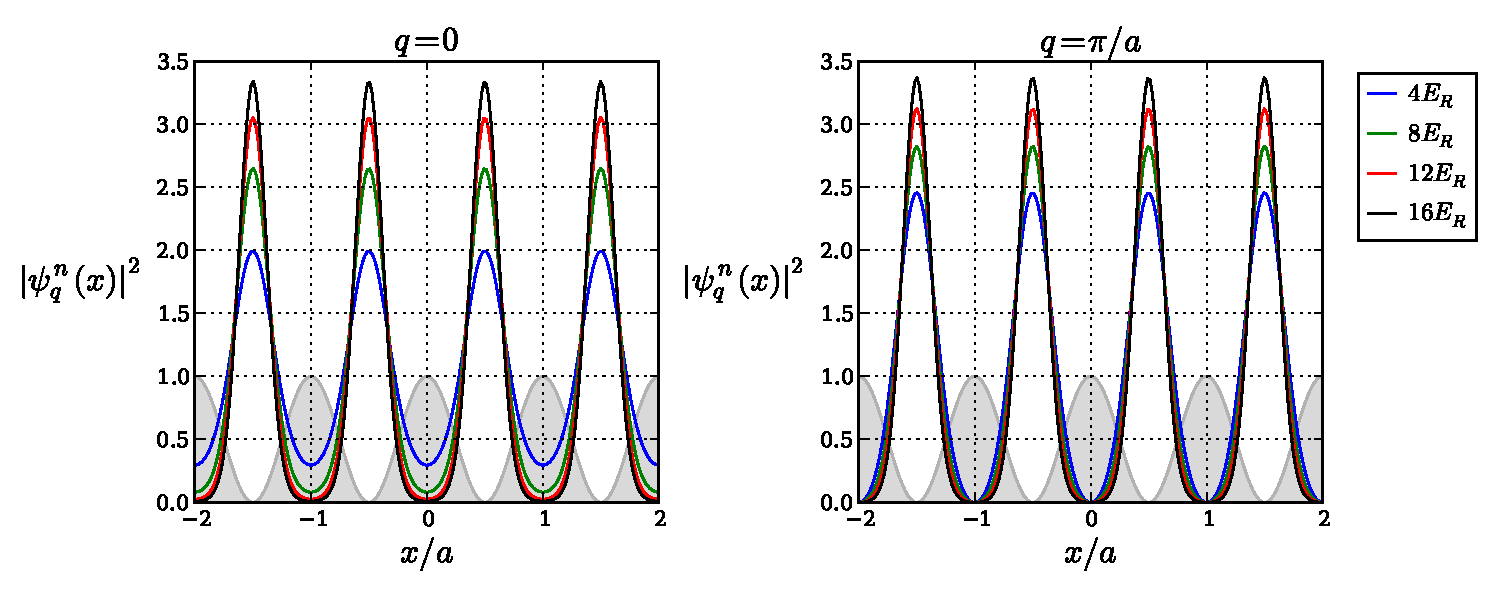
\includegraphics[width=\textwidth]{../BandStructure_figures/eigenfuns1d.pdf}
\caption[Eigenstates in 1D lattice.]{\small Eigenstates of the Hamiltonian in a 1D optical lattice shown for $q=0$ (left) and $q=\pi/a$ (right) for various lattice depths. The states are normalized so that the integral of the probability density over one lattice site is equal to one.  The gray shaded region is shown to indicate the variation of the lattice potential. }
\label{fig:eigenfuns1d}
\end{figure}

\subsection{Wannier states} 
\label{sec:1Dlattice}

It is useful to define a basis of states that are localized around a single
lattice site.  We will see later on that when using such a basis the
Hamiltonian for the Hubbard model takes its most familiar form.    The
localized states, centered around the site at $X_{j}$, can be constructed as the following superposition of
eigenstates of the Hamiltonian 
\begin{equation}
 w^{n}(x-X_{j}) =  \frac{1}{N_{\mathrm{s}}} \sum_{q}  e^{-i q X_{j} } \psi_{q}^{n}(x) 
 \label{eq:wannier}
\end{equation}
Here we have considered a finite sized lattice with a total of $N_{\mathrm{s}}$
sites,  which implies that the quasimomentum is only defined for the discrete
values $q = \frac{n}{N_{\mathrm{s}}} \frac{\pi}{a}$ where 
$ n \in \lbrace
-N_{\mathrm{s}}+1, -N_{\mathrm{s}}+2, \ldots, N_{\mathrm{s}}-1,  N_{\mathrm{s}}  \rbrace$.
Care must be taken when summing up the eigenstates to obtain the Wannier
states, since the $\psi_{q}^{n}(x)$ are defined by Eq.~\ref{eq:blochstate} up
to an overall phase factor.   We want the Wannier function to be real valued,
and to obtain such a result we must choose a phase factor for all the
eigenstates such that $\psi_{q}^{n}(x=x_{j})$ is a real number, where $x_{j}$
denotes the center of any lattice site.   Using this prescription for the
phase,  and then adding up all the eigenstates, as indicated in
Eq.~\ref{eq:wannier}, one obtains the Wannier states which are shown in
Fig.~\ref{fig:wannier1d}.   It is seen in the figure that the Wannier state
will be real valued only if $x_{j}$ is the center of a lattice site. 
\begin{figure}
\centering 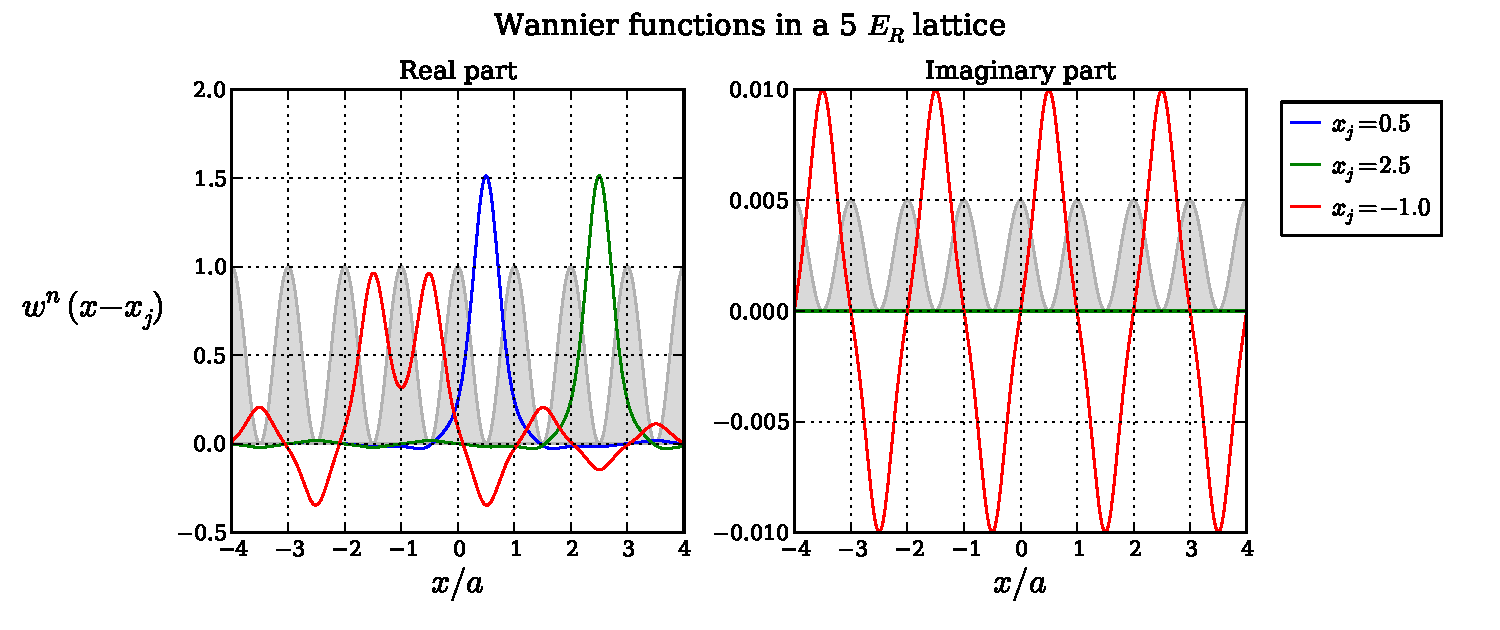
\includegraphics[width=\textwidth]{../BandStructure_figures/wannier1d.pdf}
\caption[Wannier states in 1D lattice.]{\small Localized Wannier states in a 1D
optical lattice with $\vo=5E_{R}$.  With the definition given in
Eq.~\ref{eq:wannier}, the Wannier states will be real valued if $x_{j}$ is at
the center of a lattice site.  The gray shaded region is shown to indicate the
spatial variation of the lattice potential.  } \label{fig:wannier1d}
\end{figure}

In some treatments (for instance~\cite{salomon2013many}) the Wannier function
is defined with a normalization factor of $\sqrt{N_{s}}$  rather than $N_{s}$
as shown here.   This is considering eigenfunctions $\psi_{q}^{n}(x)$ which are
normalized when integrating over the full extent in the lattice.  We stick to
the $N_{s}$ normalization factor, without the square root, since the
eigenfunctions that are obtained numerically come out normalized over a lattice
site, as was explained in the previous section. 


As the lattice depth is increased, the Wannier states become more localized.
This leads to less overlap betweeen Wannier states in adjacent sites, which
results in a reduction of the amplitude for a particle to tunnel from one site
to the next one.   More localized states also imply that the on-site
interaction will be larger, since two particles in the same site will be closer
to each other on average.   The Wannier states as a function of lattice depth
are shown in Fig.~\ref{fig:wannier1d_V0}.  
\begin{figure}
\centering 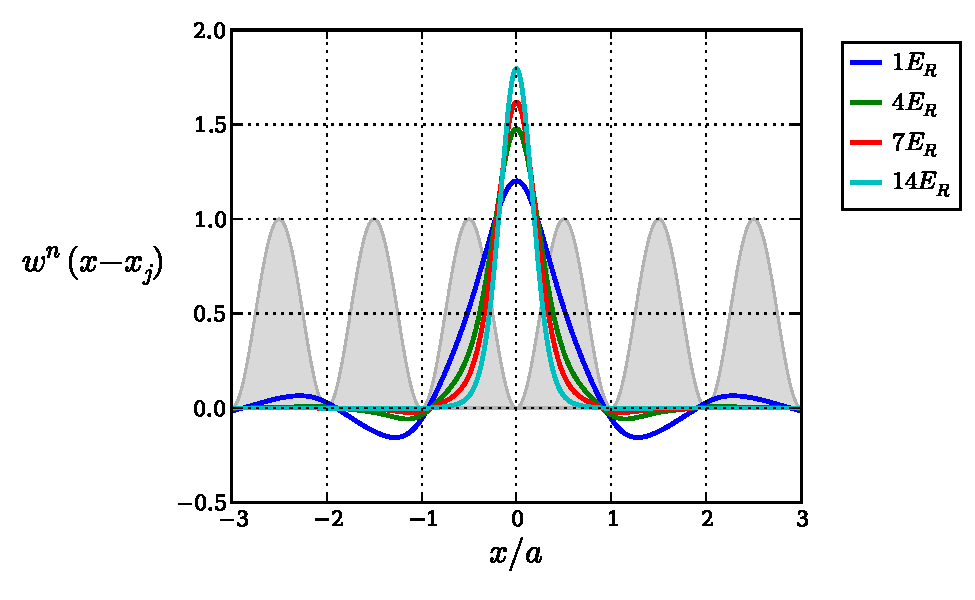
\includegraphics[width=0.6\textwidth]{../BandStructure_figures/wannier1d_V0.pdf}
\caption[Wannier states in 1D lattice for various lattice depths.]{\small Localized Wannier states in a 1D
optical lattice for various lattice depths. The gray shaded region is shown to  indicate the spatial variation of the lattice potential.
} \label{fig:wannier1d_V0}
\end{figure}


\section{Three-dimensional optical lattice potential}

The hamiltonian for an atom moving in a  3D lattice can be separated in the
three spatial coordinates.  So we can use the solutions that were obtained in
the previous section for the 1D lattice and obtain the band structure and the
Wannier states for the 3D lattice.   
The band structure is shown in Fig.~\ref{fig:bands3d_V0}. 
\begin{figure}
\centering 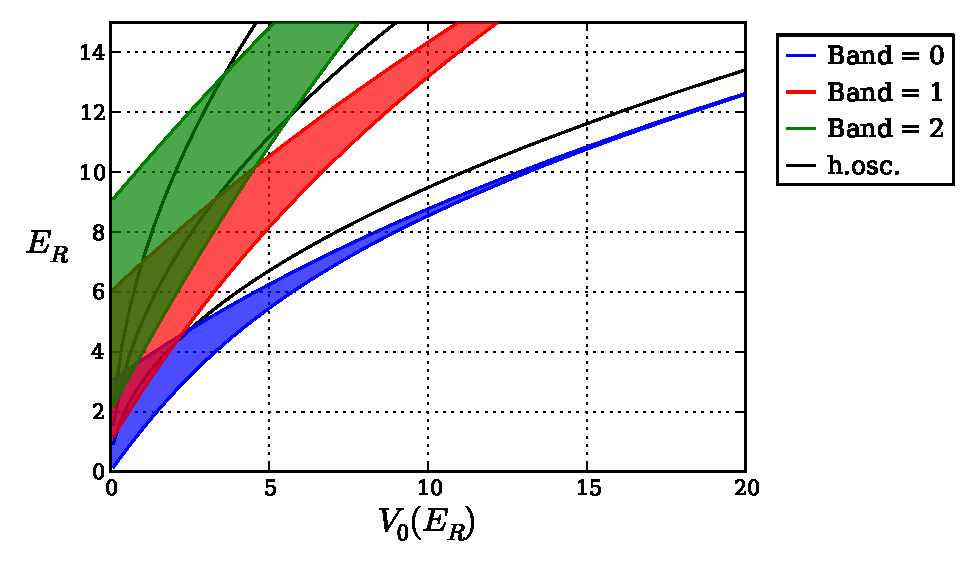
\includegraphics[width=0.6\textwidth]{../BandStructure_figures/bands3d_V0.pdf}
\caption[Band structure in 3D lattice.]{\small Band structure in a 3D optical lattice.  Each band is indicated by the colored area,  the harmonic oscillator states in an isolated lattice site are shown as black lines. }
\label{fig:bands3d_V0}
\end{figure}

The Wannier states in a 3D lattice are
simply products of the Wannier states in each of the three spatial coordinates.  They are defined as 
\begin{equation}
 w^{n}(\bv{r}-\bv{R}_{j}) =  \frac{1}{N_{\mathrm{s}}^{3}} \sum_{\bv{q}} e^{-i \bv{q}\cdot\bv{R}_{j} }
     \prod_{u=x,y,z}  \psi_{q_{u}}^{n_{u}}(u) 
 \label{eq:wannier3D}
\end{equation}
where $N_{\mathrm{s}}^{3}$ is the total number of sites in the lattice. 

\section{Hubbard Hamiltonian}

The hamiltonian for a single atom in a 3D
optical lattice is given by  
\begin{equation}
  H_{\text{single,3D}} = - \frac{\hbar^{2}}{2m} \left( \frac{\partial^{2}}{\partial x^{2}}
                            + \frac{\partial^{2}}{\partial y^{2}}
                            + \frac{\partial^{2}}{\partial z^{2}} \right)
 + \vo\left( \cos^{2}(kx)  + \cos^{2}(ky) + \cos^{2}(kz) \right)
\end{equation}
and when $N$ particles are considered, along with their interactions the hamiltonian takes a more complicated form 
\begin{equation}
\begin{split}
  H = & \sum_{l}^{N}\left[ -\frac{\hbar^{2}}{2m} \left( \frac{\partial^{2}}{\partial x_{l}^{2}}
                            + \frac{\partial^{2}}{\partial y_{l}^{2}}
                            + \frac{\partial^{2}}{\partial z_{l}^{2}} \right)
 + \vo\left( \cos^{2}(kx_{l})  + \cos^{2}(ky_{l}) + \cos^{2}(kz_{l}) \right) \right]\\
      &  + \frac{1}{2}\sum_{ l,m, l\neq m}^{N} V_{\mathrm{int}}(x_{l},x_{m} \\ 
    = & H_{0} + H_{\text{int}}
 \label{eq:hubbard1st}
\end{split} 
\end{equation} 
where the particles are labeled by indices $l$,$m$, and
$V_{\mathrm{int}}$ is the potential energy of interaction between two partcles.
In the last line we have defined the more concise notation that splits the
Hamiltonian into the non-interacting ($H_{0}$) and the interacting ($H_{\text{int}}$) parts. Solving this
problem is a daunting task primarily for two reasons:
\begin{enumerate}
    \item The Bose or Fermi statistics of the identical particles under consideration require the wavefunctions to be symmetrized or antysymmetrized products of single-particle wavefunctions.     \item The interactions between the particles prevent a straightforward reformulation of the problem as a collection of easier-to-solve single particle hamiltonians.  
\end{enumerate}

The formalism of many-body theory encapsulates a series of methods to deal with
the two issues mentioned above.   First, the reformulation of the Schrodinger
equation in the language of second quantization provides the advantage that the
statistics are automatically taken into account by the notation, so one can
essentially forget about the the (anti)symmetrization of the many-particle wave
functions.  The small price to pay is that one needs to be very careful and
consistent about the order in which operators show up in the notation, since
the symmetry properties of the resulting states are contained in the
commutation relations defined between the operators.  Furthermore, second
quantization makes it easy to consider the extended Hilbert space where the
number of particles is not fixed, this is known as Fock space. 

For weak interactions, many-body theory provides a solution to the problem in
terms of perturbation expansions for the physical quantities of interest.   The
theoretical formalism also reduces most of the important physical quantities in
terms of certain matrix elements (Green's functions) which allows the user to
concentrate on obtaining such matrix elements which serve as a starting point
for the exploration of the properties of any system.   The complication arises
when the interactions are not weak, and the perturbative approach of the
many-body formalism breaks down.   For this reason, the Hubbard model with strong
interactions (we will quantify the definition of strong later on) has been a
major challenge for theoretical physicists over the last four decades. 
 


\subsection{Second quantization}

The contents of this section follow the treatment in the books by Fetter and Walecka~\cite{fetter2003quantum} and Schwabl~\cite{schwabl2005advanced}.  

Let's start with a complete orthonormal set of single particle states $\lbrace
|i\rangle \rbrace = \lbrace |1\rangle, |2\rangle, \ldots \rbrace$, using these
states we can write the basis states for the $N$-particle system as
\begin{equation}
   | i_{1}, \ldots i_{\alpha}, \ldots i_{N} \rangle  
\end{equation} 
which represents a state in which particle 1 is in state $i_{1} \in \lbrace |i\rangle \rbrace$, particle
$\alpha$ is in state $i_{\alpha}$ and so on.   These product states are not eigenstates
of the permutation operator $P_{ij}$ which interchanges particles $i$ and $j$.
However, starting from the product states we can obtain the symmetrized (bosons) and antisymmetrized (fermions) normalized basis states.   

For bosons the normalized symmetrized states are
\begin{equation} 
  | n_{1},  n_{2}, \ldots \rangle = 
  \frac{1}{\sqrt{N!n_{1}!n_{2}!\ldots}} \sum_{P}  P | i_{1},  i_{2}, \ldots i_{N} \rangle
\end{equation} 
where the sum over $P$ runs over all $N!$ elements of the permutation group for
$N$ objects.  In this expression, $n_{1}$ is the number of times that the state
$|1\rangle$ occurs among the $N$ particles,  or in other words, $n_{1}$ is the number of
particles in state $|1\rangle$.  The sum of all occupation numbers $n_{i}$ must equal the total number of particles, but otherwise there is no restriction in the occupation number for bosons.

For fermions the normalized antysymmetrized states are written in the form of Slater determinants:
\begin{equation}
\begin{split}
  | n_{1},  n_{2}, \ldots \rangle = &
  \frac{1}{\sqrt{N!}} \sum_{P} (- 1)^{P} P | i_{1},  i_{2}, \ldots i_{N} \rangle \\
  = &
  \frac{1}{\sqrt{N!}}
  \begin{vmatrix}
  |i_{1}\rangle_{1} & |i_{1}\rangle_{2} & \dotsm & |i_{1}\rangle_{N} \\
  \vdots &  \vdots &  \ddots   & \vdots \\
  |i_{N}\rangle_{1} & |i_{N}\rangle_{2} & \dotsm & |i_{N}\rangle_{N} \\
\end{vmatrix}
\end{split} 
  \label{eq:antisymmetrize} 
\end{equation}  
In this case, the product states are multiplied by -1 for odd permutations, and the occupation numbers $n_{i}$ can only take the values 0 or 1. 

For both bosons and fermions, we can combine the states for $N=0,1,2,\ldots$ particles to
obtain a complete orthonormal set of states for arbitrary particle number.
This set of states, which are referred to as number states, spans what is called the Fock space.   

We now define the 
creation  operators for bosons, which allow us to take a state from the
subspace of $N$ particles, to the subspace of $N+1$  particles. 
\begin{equation}
 a_{i}^{\dagger} | \ldots, n_{i}, \ldots \rangle  = \sqrt{n_{i}+1}|\ldots, n_{i}+1, \dots\rangle
\end{equation}
It follows that the adjoint of the creation operator is the annihilation operator and satisfies
\begin{equation}
a_{i} | \ldots, n_{i}, \ldots \rangle  
=\begin{cases}
\sqrt{n_{i}}|\ldots, n_{i}-1, \dots\rangle
& \text{if $n_{i}\geq 0$},\\
0 & \text{if $n_{i}=0$}
\end{cases}
\end{equation}
The creation and annihilation operators are defined such that one can create any state
starting from the vacuum state $|0\rangle \equiv |0,0,\ldots\rangle$ in which
there are no particles at all.  In more formal terms 
\begin{equation}
  | n_{1}, n_{2}, \dots \rangle = \frac{1}{\sqrt{n_{1}!n_{2}!\ldots}} 
   ( a_{1}^{\dagger} ) ^{n_{1}}  
   ( a_{2}^{\dagger} ) ^{n_{2}}  \ldots | 0 \rangle
  \label{eq:numberstate}
\end{equation}
The boson creation and annihilation operators satisfty the Bose communtation relations
\begin{equation}
  [a_{i}, a_{j}] = 0 \ \ \ \ \  [a_{i}^{\dagger}, a_{j}^{\dagger}] = 0 \ \ \ \ \   [a_{i},a_{j}^{\dagger}]=\delta_{ij}
\end{equation}

In the case of fermions we want to also define creation  operators such that
the number states can be written as in Eq.~\ref{eq:numberstate}.    A subtlety
arises in the case of fermions since  the order in which the
creation operators are applied affects the resulting number state\footnote{This is
not a problem in bosons which is seen by looking at Eq.~\ref{eq:numberstate}
and recalling that the Bose commutation relations say that all creation
operators commute}.   Take the number state defined in Eq.~\ref{eq:antisymmetrize}.
If we interchange the state labels 1 and 2 we get 
\begin{equation}
\begin{split}
  | n_{2},  n_{1}, \ldots \rangle = &
  \frac{1}{\sqrt{N!}} \sum_{P} (- 1)^{P} P | i_{2},  i_{1}, \ldots i_{N} \rangle \\
   = & -
  \frac{1}{\sqrt{N!}} \sum_{P} (- 1)^{P} P | i_{1},  i_{2}, \ldots i_{N} \rangle \\ 
   = & -
  | n_{1},  n_{2}, \ldots \rangle 
\end{split}
\label{eq:fermionsign}
\end{equation} 
where the minus sign in the second line is a result of the properties of determinants, namely you get a minus sign if you exchange two columns. 

If we adopt as a definition of the creation operators the following expression for the number state 
\begin{equation}
  | n_{1}, n_{2}, \dots \rangle =  
   ( a_{1}^{\dagger} ) ^{n_{1}}  
   ( a_{2}^{\dagger} ) ^{n_{2}}  \ldots | 0 \rangle \ \ , \ \ \ \ n_{i}=0,1 
  \label{eq:numberstateFermions}
\end{equation}
then using the result of Eq.~\ref{eq:fermionsign} above, the fermion creation operators must satisfy the following anticommutation relation
\begin{equation}
 a_{i}^{\dagger}a_{j}^{\dagger} + a_{j}^{\dagger}a_{i}^{\dagger} \equiv [a_{i}^{\dagger}, a_{j}^{\dagger}]_{+} = 0 
\end{equation}
Notice that this also contains the necessary implication that $(a_{i}^{\dagger})^{2}=0$, which is a manifestation of the Pauli exclusion principle.  It follows from here that the creation and annihilation operators for fermions satisfy 
\begin{equation}
\begin{split}
  a_{i}^{\dagger}| \ldots, n_{i}, \ldots \rangle 
  =  & (1-n_{i})(-1)^{\sum_{k<i} n_{k}} | \ldots, n_{i}+1, \ldots \rangle \\
  a_{i}| \ldots, n_{i}, \ldots \rangle 
  =  & n_{i}(-1)^{\sum_{k<i} n_{k}} | \ldots, n_{i}-1, \ldots \rangle
\end{split} 
\end{equation}
and also that they satisfy the Fermi anticommutation relations 
\begin{equation}
  [a_{i}, a_{j}]_{+} = 0 \ \ \ \ \  [a_{i}^{\dagger}, a_{j}^{\dagger}]_{+} = 0 \ \ \ \ \   [a_{i},a_{j}^{\dagger}]_{+}=\delta_{ij}
\end{equation}

From now on we shall focus on the case of Fermions, since this is the most
relevant for our experiment.  

\subsection{Operators in second quantization}

So far two great leaps have been taken: 
\begin{enumerate}
 \item We have
swept antisymmetrization under the rug by introducing the number states,
defined from the vacuum in terms of creation operators wich satisfy the Fermi anticommutation reations.  
 \item We started from an $N$ particle hamiltonian, but we have now defined states that can handle the description of systems with an arbitrary number of particles 
\end{enumerate}
The two ideas mentioned are related to the states used to describe the system, now we will turn to the problem of the observables and see how they are handled in the second quantization.  


Let us consider the following sum over particles $\sum_{\alpha}
|i\rangle_{\alpha} \langle j | _{\alpha} $ and apply it to the number states as
defined in Eq.~\ref{eq:antisymmetrize}
\begin{equation}
  \left(
   \sum_{\alpha} |i\rangle_{\alpha} \langle j | _{\alpha}  \right)
  | n_{1},  n_{2}, \ldots \rangle = 
  \frac{1}{\sqrt{N!}} \sum_{P} (- 1)^{P} P 
  \left( \sum_{\alpha} |i\rangle_{\alpha} \langle j | _{\alpha} 
   | i_{1},  i_{2}, \ldots i_{N} \rangle \right)
\end{equation}
On the left hand side, for the term in parenthesis not to vanish, there must be one particle in state
$|j\rangle$, so we must have $n_{j}=1$ in the initial state.  Also, since these are fermions, there can be no
particles in state $|i\rangle$ in the intitial state, so $n_{i}=0$,  or else the
Slater determinant operator will make the state
vanish after applying the $|i\rangle\langle j|$.  If the particle initially in state $|j\rangle$ is labeled as  $\beta$  then the two mentioned 
conditions can be embodied as 
\begin{equation}
\begin{split}
  \left(
   \sum_{\alpha} |i\rangle_{\alpha} \langle j | _{\alpha}  \right)
  | n_{1},  n_{2}, \ldots \rangle = &
   n_{j}(1-n_{i}) 
  \frac{1}{\sqrt{N!}} \sum_{P} (- 1)^{P} P \left( 
    |i\rangle_{\beta}\underbrace{ 
   | i_{1},  i_{2}, \ldots i_{N} \rangle}_{\text{wihtout }|j\rangle_{\beta}}  \right) \\
   =&  n_{j}(1-n_{i})
  \frac{1}{\sqrt{N!}}
  \begin{vmatrix}
  |i_{1}\rangle_{1} & |i_{1}\rangle_{2} & \dotsm & |i_{1}\rangle_{N} \\
  \vdots &  \vdots &     & \vdots \\
  |i\rangle_{1} & |i\rangle_{2} & \dotsm & |i\rangle_{N} \\
  \vdots &  \vdots &     & \vdots \\
  |i_{N}\rangle_{1} & |i_{N}\rangle_{2} & \dotsm & |i_{N}\rangle_{N} \\
\end{vmatrix} \\
\end{split} 
\end{equation}
In the determinant of the left the state $|i\rangle$ appears in the $j^{\text{th}}$ row, so a few rows need to be exchanged to put it in the correct place according to our sign convention for the number states.  
\begin{equation}
\begin{split}
  \left(
   \sum_{\alpha} |i\rangle_{\alpha} \langle j | _{\alpha}  \right)
  | n_{1},  n_{2}, \ldots \rangle = &
  n_{j}(1-n_{i})| \ldots, n_{i}+1, \ldots,  n_{j}-1, \ldots  \rangle \times  
 \begin{cases}
(-1)^{\sum_{k<j} n_{k} + \sum_{k<i}n_{k}  }
& \text{if $i\leq j$},\\
(-1)^{\sum_{k<j} n_{k} + \sum_{k<i}n_{k} -1 } & \text{if $i>j$}
\end{cases}  \\
   = &  a_{i}^{\dagger} a_{j} 
  | n_{1},  n_{2}, \ldots \rangle 
\end{split} 
\end{equation}
where the last equality can be obtained by examining the definition of the creating and annihilation operators given above. 

After this last step we can establish the important relation
\begin{equation}
   \sum_{\alpha} |i\rangle_{\alpha} \langle j | _{\alpha} = 
     a_{i}^{\dagger} a_{j} 
\end{equation}

We now turn our attention to the operators in the $N$-particle system.  Consider an operator $T$ that is a sum over single particle operators 	
\begin{equation}
  T = \sum_{\alpha} t_{\alpha}
\end{equation}  
If we insert the completness relation for the single particle states twice in this sum we have 
\begin{equation}
\begin{split}
  T = & \sum_{\alpha} \left( \sum_{i} |i\rangle_{\alpha}\langle i |_{\alpha} \right)
        t_{\alpha} \left( \sum_{j} |j\rangle_{\alpha}\langle j |_{\alpha} \right) \\
    = & \sum_{ij}   \langle i | t | j \rangle  \sum_{\alpha} |i\rangle_{\alpha} \langle j |_{\alpha} \\ 
    = & \sum_{ij}   \langle i | t | j \rangle a_{i}^{\dagger} a_{j} \equiv \sum_{ij} t_{ij}   a_{i}^{\dagger} a_{j} 
\end{split}  
\end{equation}

This is the other big leap provided by the second quantization:  the operators
which were written as a sum over particles now are written as a sum of creation
and annihilation operators over single particle states.   

Operators like the
potential energy, which are a sum over
two-particle (or many-particle) operators,  can be equally expressed as sums of creation and annihilation operators.  For a two-body operator we have the expression
\begin{equation}
\begin{split}
F = & \frac{1}{2} \sum_{\alpha\neq\beta} f(\bv{x}_{\alpha}, \bv{x}_{\beta} )  \\
  = & \frac{1}{2} \sum_{ijkm} \langle ij | f | km \rangle a_{i}^{\dagger} a_{j}^{\dagger} a_{m} a_{k} 
\end{split}
\end{equation}

\subsection{Second quantized Hubbard hamiltonian}

The Hubbard hamiltonian in Eq.~\ref{eq:hubbard1st} is a sum of two single-particle operators and one two-particle operator.  These are respectively: the kinetic energy, the energy of the atoms in the lattice potential, and the interactions between the atoms.  As a single-particle basis we pick the Wannier states that were derived in Section.~\ref{sec:1Dlattice}

In the Hubbard hamiltonian the two single-particle operators are grouped together to define the non-interacting part of the hamiltonian
\begin{equation}
\begin{split}
  H_{0} = & \sum_{l}^{N} -\frac{\hbar^{2}}{2m} \left( \frac{\partial^{2}}{\partial x_{l}^{2}}
                            + \frac{\partial^{2}}{\partial y_{l}^{2}}
                            + \frac{\partial^{2}}{\partial z_{l}^{2}} \right)
 + \vo\left( \cos^{2}(kx_{l})  + \cos^{2}(ky_{l}) + \cos^{2}(kz_{l}) \right) \\
       = & \sum_{l}^{N} H_{\text{single,3D}}^{l}
\end{split}
\end{equation}

\subsubsection{Tunneling matrix element, $t$}
$H_{0}$ is a single particle operator, so it's second quantized form is 
\begin{equation}
\begin{split}
  H_{0} = & \sum_{ij} \langle i| H_{\text{single,3D}} |j \rangle a_{i}^{\dagger} a_{j} \\
        = & -\sum_{ij} t_{ij}  a_{i}^{\dagger} a_{j} \\
\end{split}
\end{equation}  
Note that the sign of $t_{ij}$ was picked rather arbitrarily to follow the
usual conventions.  We now proceed to find the value of the matrix element.
We use the definition of the Wannier states given in Eq.~\ref{eq:wannier3D} to
find 
\begin{equation}
\begin{split}
-t_{ij}  
= & 
  \frac{1}{N_{\mathrm{s}}^{6}}\int \mathrm{d}\bv{r}\ 
     \sum_{\bv{q}'} e^{i \bv{q'}\cdot\bv{R}_{i} }
     \prod_{u'=x,y,z}  \psi_{q'_{u'}}^{n'_{u'}*}(u') 
  \Big( H_{\text{single,3D}}  \Big)
     \sum_{\bv{q}} e^{-i \bv{q}\cdot\bv{R}_{j} }
     \prod_{u=x,y,z}  \psi_{q_{u}}^{n_{u}}(u)\\ 
= &
  \sum_{\bv{q}\bv{q}'}   
  \frac{E_{\bv{q}}^{n}}{N_{\mathrm{s}}^{6}}
   e^{ i \bv{q}'\cdot\bv{R}_{i} }  e^{ -i \bv{q}\cdot\bv{R}_{j} }
   \int\mathrm{d}\bv{r}\ 
     \prod_{u'=x,y,z}  \psi_{q'_{u'}}^{n'_{u'}*}(u') 
     \prod_{u=x,y,z}  \psi_{q_{u}}^{n_{u}}(u) \\ 
= &
  \sum_{\bv{q}\bv{q}'}   
  \frac{E_{\bv{q}}^{n}}{N_{\mathrm{s}}^{6}}
   e^{ i \bv{q}'\cdot\bv{R}_{i} }  e^{ -i \bv{q}\cdot\bv{R}_{j} }
   \delta_{\bv{q}\bv{q}'} \delta_{nn'} N_{\mathrm{s}}^{3} \\
= &
  \frac{1}{N_{\mathrm{s}}^{3}}
  \sum_{\bv{q}}   E_{\bv{q}}^{n}
   e^{ i \bv{q}\cdot(\bv{R}_{i} - \bv{R}_{j}) } \\
\end{split} 
\end{equation}
We observe that there is no amplitude to go between states that are in two different bands, as is indicated by the appereance of $\delta_{nn'}$.   In what follows we will consider only the lowesrt band, $n=0$,  so we will drop the band index altogether.  This simplification imposes two important requirements for our system:
\begin{enumerate}
\item The temperature needs to be small compared to the energy gap between the lowest and first excited band.   
\item The interaction enrgy scale must also be small comapred to the energy gap between the lowest and first excited band. 
\end{enumerate}

In the 3D lattice, the energy $E_{\bv{q}} = \sum_{u=x,y,z} E_{q_{u}}^{u} $, and by inserting this into the sum for $t_{ij}$ above we find 
\begin{multline}
-t_{ij} =  \frac{1}{N_{\mathrm{s}}^{3}} \left[ 
          \left(\sum_{q_{x}} E_{q_{x}}^{\text{\tiny 1D}}   e^{ i q_{x} x_{ij} }   \right)
          \sum_{q_{y}} e^{ i q_{y} y_{ij} }   
          \sum_{q_{z}} e^{ i q_{z} z_{ij} }  
   \right. \\
\left. 
          + 
          \sum_{q_{x}} e^{ i q_{x} x_{ij} }  
          \left(\sum_{q_{y}} E_{q_{y}}^{\text{\tiny 1D}}   e^{ i q_{y} x_{ij} }   \right)
          \sum_{q_{z}} e^{ i q_{z} z_{ij} }  
          + 
          \sum_{q_{x}} e^{ i q_{x} x_{ij} }  
          \sum_{q_{y}} e^{ i q_{y} y_{ij} }   
          \left(\sum_{q_{z}} E_{q_{z}}^{\text{\tiny 1D}}   e^{ i q_{z} z_{ij} }   \right)
\right]
\end{multline}
We make use of the identity $\sum_{q_{x}} e^{ iq_{x}(x_{i}-x_{j}) } = N_{\mathrm{s}} \delta_{x_{i}x_{j}}$, and similarly for $y,z$ to obtain
\begin{equation}
-t_{ij} =  \frac{1}{N_{\mathrm{s}}} \left[ 
          \left(\sum_{q_{x}} E_{q_{x}}^{\text{\tiny 1D}}   e^{ i q_{x} x_{ij} }   \right)
          \delta_{y_{i}y_{j}}
          \delta_{z_{i}z_{j}}
          + 
          \left(\sum_{q_{y}} E_{q_{y}}^{\text{\tiny 1D}}   e^{ i q_{y} x_{ij} }   \right)
          \delta_{x_{i}x_{j}}
          \delta_{z_{i}z_{j}}
          + 
          \left(\sum_{q_{z}} E_{q_{z}}^{\text{\tiny 1D}}   e^{ i q_{z} z_{ij} }   \right)
          \delta_{x_{i}x_{j}}
          \delta_{y_{i}y_{j}}
\right]
\end{equation}

We see that if $i=j$ we have 
\begin{equation}
  -t_{ii} =  \frac{3}{N_{\mathrm{s}}} 
          \sum_{q} E_{q}^{\text{\tiny 1D}}  
\end{equation}
Considering this term just adds an overall energy (proportional to the number
of particles in the system) to the hamiltonian, so we just ignore it for
convenience.  If on the other hand $i\neq j$, then we see that we can only
consider the posibility that one of the $x_{ij}, y_{ij}, z_{ij}$ is non-zero,
otherwise all three of the terms in the expression above will vanish
due to the Kronnecer delta terms. 

It is interesting to see that there is no matrix elemnt to tunnel 
diagonally between sites in the 3D lattice.  
This is in contrast to  the
actual situation in real materials, where localized atomic orbitals will adopt
functional forms that have nothing to do with the Wannier state.  In such cases
there is generally a matrix element for an electron to
tunnel between orbitals that are localized in any two lattice sites.
Tunneling beyond nearest neighbors is typically neglected in what is called the
tight-binding limit.

For the 3D lattice the expression for the tunneling matrix elements simplifies to 
\begin{equation}
  t_{ij} = -\frac{1}{N_{\mathrm{s}}} \sum_{q} E_{q}^{\text{\tiny 1D}} e^{iq \Delta_{ij}} 
\end{equation}
where $\Delta_{ij}$ is the distance between sites at $\bv{R}_{i}$ and $\bv{R}_{j}$, and $R_{ij}$ must be purely directed along $x$, $y$, or $z$.  Also, as in the definition of the 1D Wannier states, the sum over $q$ runs over the discrete
values $q = \frac{n}{N_{\mathrm{s}}} \frac{\pi}{a}$ where 
$ n \in \lbrace
-N_{\mathrm{s}}+1, -N_{\mathrm{s}}+2, \ldots, N_{\mathrm{s}}-1,  N_{\mathrm{s}}  \rbrace$.

We see that $t_{ij}$ and $E_{q}^{\text{\tiny 1D}}$ are the Fourier series of one another, or in other words that the relation just shown can be inverted to obtain
\begin{equation} 
  E_{q}^{\text{\tiny 1D}} = - \sum_{\Delta_{ij}} t_{ij} e^{-iq \Delta_{ij}} 
\end{equation}
In the tight-binding approximation $\Delta_{ij} \in \lbrace -a, a \rbrace$ and $t_{ij}\equiv t$, so we have
\begin{equation}
  E_{q,\text{tb}}^{\text{\tiny 1D}} = -2 t\cos( qa) 
\end{equation}

It is useful to find out the range of lattice depths for which the
tight-binding approximation is valid in the optical lattice potential.  To do
this we just need to look at the tunneling matrix elements for beyond
nearest-neighbor tunneling,  this is shown in Fig.~\ref{fig:tightbinding},
which shows that for lattice depths $\gtrsim 5 E_{R}$  we can safely ignore
tunneling beyond nearest neighbors.  
\begin{figure}
\centering 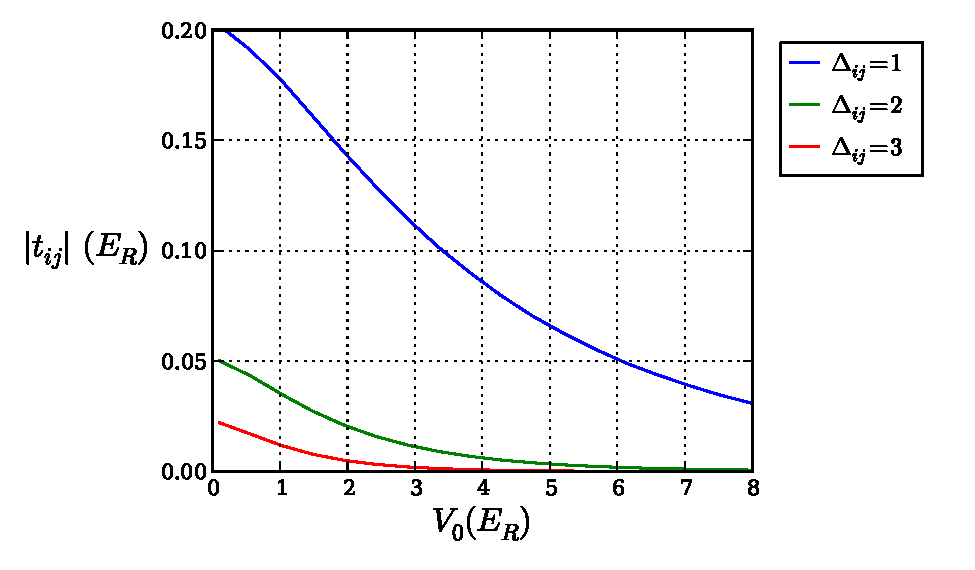
\includegraphics[width=0.6\textwidth]{../BandStructure_figures/tightbinding_V0_interp.pdf}
\caption[Tunneling matrix elements in a 3D lattice.]{\small Tunneling matrix
element in an optical lattice as a function of lattice depth.  Nearest-neighbor
and beyond nearest neighbor matrix elements are shown to illustrate the range
of lattice depths for which the tight-binding limit is a good approximation.
$X_{ij}$ corresponds to the distance between intial and final site in the tunneling matrix element. 
 } \label{fig:tightbinding}
\end{figure}

Finally, we have the second quantized form of $H_{0}$ in the tight-binding limit
\begin{equation}
  H_{0} = -t \sum_{ \langle ij \rangle } a_{i}^{\dagger}a_{j} 
\end{equation}
where the $\langle \rangle$ denote nearest-neighbors, and the creation operator $a_{i}^{\dagger}$ create particles in the Wannier state localized at site $i$.

Notice that up to now we have ignored the spin part of the wavefunction.   We
can include it easilly by noticing that $H_{0}$ does not act on the spin at
all, so the states $|i\rangle$ and $|j\rangle$ that we have used in the
derivation above need to have the same spin.   Including the spin our basis set
is now larger, so we include it in the sum.   
\begin{equation}
  H_{0} = -t \sum_{ \langle ij \rangle, \sigma=\dbl   } a_{i\sigma}^{\dagger}a_{j\sigma} 
\end{equation}

\subsubsection{On-site interaction energy, $U$}
 

\subsection{On-site interactions} 

\section{Local density approximation }



 

\bibliographystyle{osa}
\bibliography{lattice_lda}

\end{document}




